\documentclass[11pt]{scrartcl}
\usepackage{ucs}
\usepackage{float}
\usepackage[utf8x]{inputenc}
\usepackage{ngerman}
\usepackage{amsmath,amssymb,amstext}
\usepackage{graphicx}
\usepackage{tabularx}
\usepackage[square]{natbib}
\usepackage[justification=RaggedRight, singlelinecheck=false]{caption} 
\usepackage{fancyhdr}

\pagestyle{fancy}
\lfoot{Philipp Adler}
\rfoot{\today{}}

\title{Sicherheit}
\author{Philipp Adler}
\date{\today{}}

\begin{document}

\maketitle
\tableofcontents
\pagebreak

\section{Grundlagen Securityverfahren}
\label{sec:basics-security-process}
% Moderne Kryptographie 2

\subsection{Verschlüsselungsarten}
\label{sec:ciphering types}

\subsection{Kommunikationsszenarien}
\label{sec:communication-scenarios}

\subsection{Sicherheitsziele}
\label{sec:security goals}

\subsection{Bedrohungsszenarien}
\label{sec:threat scenarios}


\section{Symmetrische Verschlüsselung}
\label{sec:symetric-ciphering}
Die symmetrische Verschlüsselung reicht bis in die Antike. Damals wussten nur die Adressierten von dem Geheimnis, nach welchem Verfahren die Botschaft verschlüsselt wurde. Cäsar zum Beispiel verschob jeden Buchstaben um 4 Stellen. So wurde aus Hallo Kdoor. Aus diesem Verschlüsselungsalgorithmus entstanden zum einen Blockchiffren, auf den ich in dem folgenden Kapitel näher eingehen werde und die Stromchiffren.\cite{1}

\subsection{Blockchiffre}
\label{sec:blockchiffre}
% Praktische Kryptographie unter Linux 2.3
% Sicherheit und Kryptographie im Internet 1.4.2
Blockchiffren teilen die Nachricht, die verschlüsselt werden soll, in eine fixe Anzahl an Blöcken, die entweder 64 oder 128 Bit groß sind. Typische, bekannte Blockchiffre sind Data Encryption Standard, Advanced Encryption Standard und International Data Encryption Algorithm.\cite{1}
\subsubsection{Der Data Encryption Standard - DES}
\label{sec:data-encryotion-standard}
\grqq{}DES wurde 1977 vom amerikanischen 'National Institute of Standards and Technologies (NIST)' veröffentlicht.\grqq{} \cite{1} Bei diesem Verfahren wird eine Blocklänge von 64 Bit und ein DES-Schlüssel von 56 Bits plus 8 \grqq{}Parity Check Bits\grqq{} \cite{1} eingesetzt. Die ersten 56 Bits werden immer zufällig generiert, wobei die letzten 8 Bits dafür sorgen, dass keine Übertragungsfehler auftreten. Da 56 Bit zufällig sind, können daraus 2\textsuperscript{56} Schlüsseln erzeugt werden. 16 Runden wird ein Block in einen 64 Bit großen Ausgabeblock umgewandelt. Bei jedem Durchgang wird ein anderer Schlüssel für die Verschlüsselung angwendet.
\cite{1}\cite{4}

\noindent \textbf{Das Schema}\\
Beim Verschlüsselungsverfahren wird der Klartext in Blöcke umgewandelt, welche alle jeweils eine Länge von 64 Bit haben, Eingangspermutation IP. Dieser Block wird dann nochmals zerlegt, sodass daraus 2 mal 32 Bit Blöcke entstehen. Der Data Encryption Standard besteht aus 16 Runden. In jeder Runde wird auf die rechte Hälfte ein Verschlüsselungsalgorithmus \textit{f} angewendet.\\
\textit{f} ist in unserem Fall die Rundenfunktion, welche aus 56 zufälligen Bits 48 Bits auswählt. Diese werden mit den 32 Bit der rechten Hälfte, die auf 48 Bit expandiert wurden, mittels XOR-Gatter verknüpft. Die 32 Bit Blöcke werden in 4 aufgeteilt und bekommen zusätzlich am Rand die Nachbarbit. \\
\begin{figure}[H]
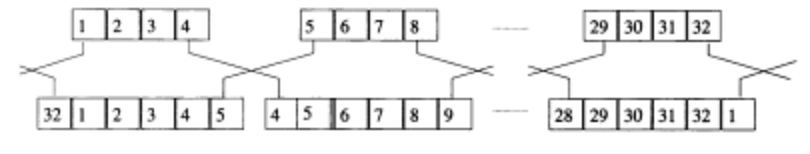
\includegraphics[width=0.60\textwidth]{Bilder/DES/DES_Expansionsabbildung}
	\caption{Expansionsabbildung des DES \citep{2}}
	\label{fig1}
\end{figure}
\noindent \grqq{}Die resultierenden 48 Bits werden in acht Blöcke zu je sechs Bits aufgeteilt\grqq{} \cite{2}, welche als Input für das S-Boxen angewandt werden. Die Substitution-Box besteht aus einer 4 * 16 Matrix, \grqq{}wobei in jeder Zeile eine Permutation der Zahlen von 0,...,15 steht.\grqq{} \citep{2} Die beiden Randbit der Blöcke entscheiden die Zeile und der Rest, die inneren Bit der Blöcke, die Spalte der Substitution-Box. Die ausgewählte Zahl wird dann binär als 4 Bit Block angegeben.\cite{2}
\begin{figure}[H]
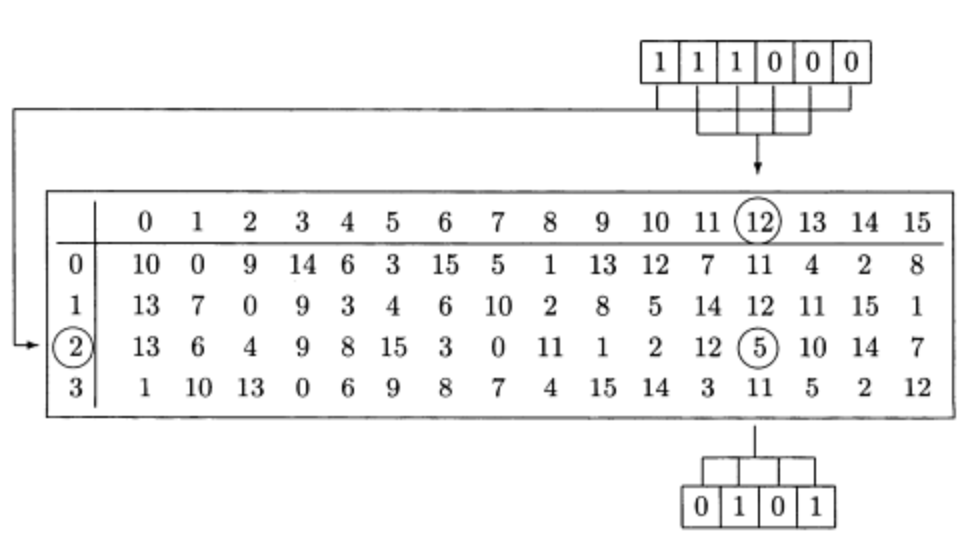
\includegraphics[width=0.45\textwidth]{Bilder/DES/S-Box}
	\caption{S-Box\citep{2}}
	\label{fig2}
\end{figure}
\noindent Da wir nun wieder acht Blöcke zu je 4 Bit haben, können diese zu 32 Bit zusammengefasst werden.\cite{2}
\begin{figure}[H]
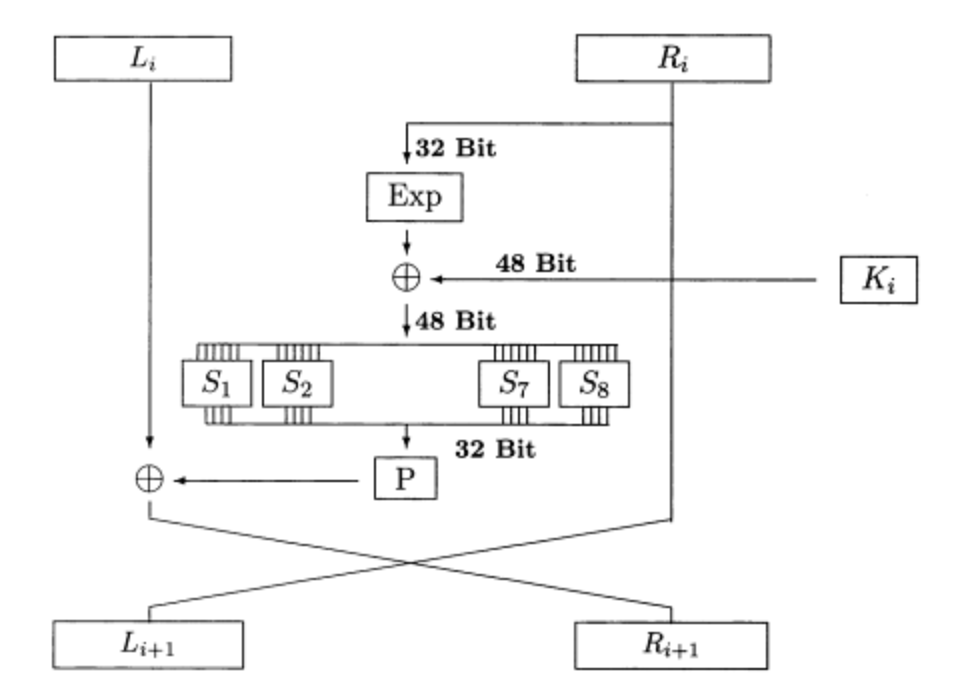
\includegraphics[width=0.45\textwidth]{Bilder/DES/DES_Rundenfunktion}
	\caption{Die DES-Rundenfunktion \citep{2}}
	\label{fig3}
\end{figure}
\noindent Das daraus resultierende Ergebnis wird nochmals permutiert und bitweise mit einem XOR-Gatter mit der linken Hälfte verknüpft und \grqq{}bildet die rechte Seite der neuen Runde.\grqq{} Unter permutiert versteht man, dass jedes einzelne bit als Zahl dargestellt wird und mit 8 addiert wird.\cite{2}
\begin{figure}[H]
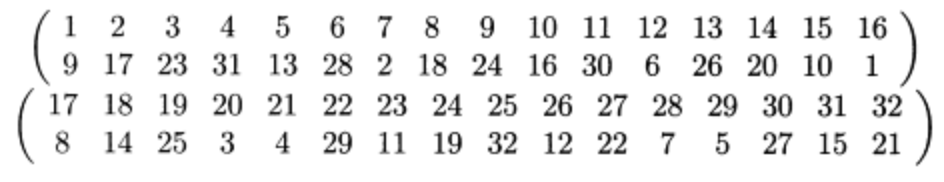
\includegraphics[width=0.40\textwidth]{Bilder/DES/DES_Permutation}
	\caption{Permutation de DES \citep{2}}
	\label{fig4}
\end{figure}
\noindent 
Da der 48 Bit Schlüssel, welcher vom 56 Bit-Hauptschlüssel hergeleitet wird, bei jeder Runde ein anderer ist, muss dieser irgendwie generiert werden. Der Hauptschlüssel wird permutiert und die Funktion PC-1 teilt diesen in 2 Blöcke zu je 28 Bit. Bei der Permutierung werden die 8 Paritätsbit entfernt, die Bits mit der Nummer 8, 16, 24, 32, 40, 48, 56, 64, wobei nur noch 56 Bit übrig bleiben. Jede der beiden Hälften wird bei jeder Iteration zirkulärisch links für die Verschlüsselung, nach rechts für die Entschlüsselung gesshiftet. Das heißt, dass jeder Block entweder ein oder zwei Bit nach links rotiert und auf 24 Bit extrahiert wird. So kann es nicht vorkommen, dass ein Rundenschlüssel nicht zweimal angewendet wird.\\
\grqq{}Nach 16 Runden werden die 64 Bit einer Ausgangspermutation unterzogen\grqq{} \cite{2}, woraus der Geheimtext resultiert. Die Ausgangspermutation ist die inverse von der Eingangspermutation, dass heißt alle 64 Bit Blöcke werden zu einem Geheimtext zusammengeführt. Nachteil dieser Implementierung ist, dass die Ein- und Ausgangspermutation öffentlich sind und so von Angreifern berechnet werden können, was die Sicherheit drastisch verringert.
\cite{2}\cite{4}
\begin{figure}[H]
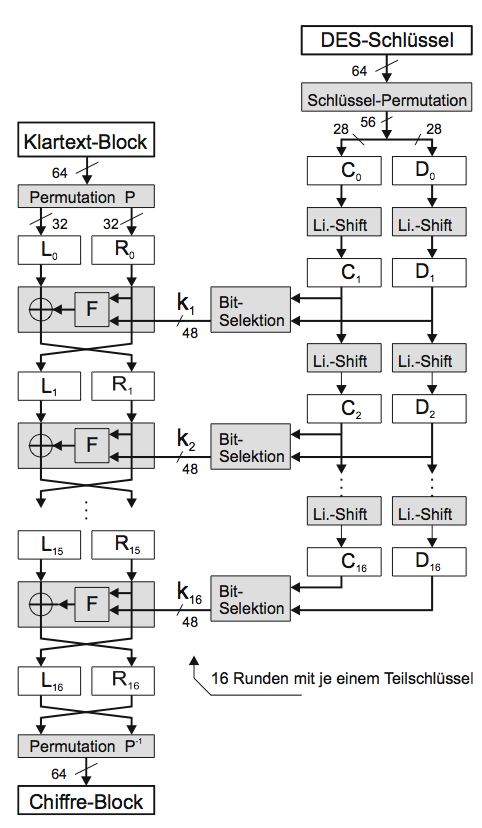
\includegraphics[width=0.40\textwidth]{Bilder/DES/DES_Schema}
	\caption{DES-Verschlüsselung-Schema \citep{3}}
	\label{fig5}
\end{figure}
% Kryptografie in Theorie und Praxis 7.6
% Kryptograhie und IT-Sicherheit 2.2
% Verteilte Systeme S.427

\subsubsection{Der Advanced Encryption Standard - AES}
\label{sec:advanced-encryotion-standard}
Da der DES-Algorithmus aus einen verhältnismäßig kurzen 56-Bit Schlüssel besteht und dieser 1999 durch einen sogenannten Brute-Force-Angriff in 22 Stunden geknackt wurde, müssen andere Vorschläge her. Die Alternative hieß AES, Advanced Encryption Standard, ist ebenfalls eine symmetrische Block-Chiffre, mit einer Blocklänge von 128 Bit.
\cite{3}

\noindent \textbf{Das Schema}\\
Der Unterschied zum DES ist, dass AES eine flexible Block- und Schlüssellänge besitzt. Der Standard besitzt eine standardisierte Blocklänge von 128 Bit und Schlüssellängen von 128 Bit, 192 Bit und 256 Bit. Wieviele Runden absolviert werden hängt von der Schlüssellänge ab. 10 Runden bei einer Schlüssellänge von 128 Bit, was derzeit der Standard ist, 12 Runden bei 192 Bit und 14 Runden bei 256 Bit. \grqq{}Vor der ersten Runde wird ein Rundenschlüssel mit dem Klartext XOR-verknüpft.\grqq{}\citep{2}
\cite{3}
\begin{figure}[H]
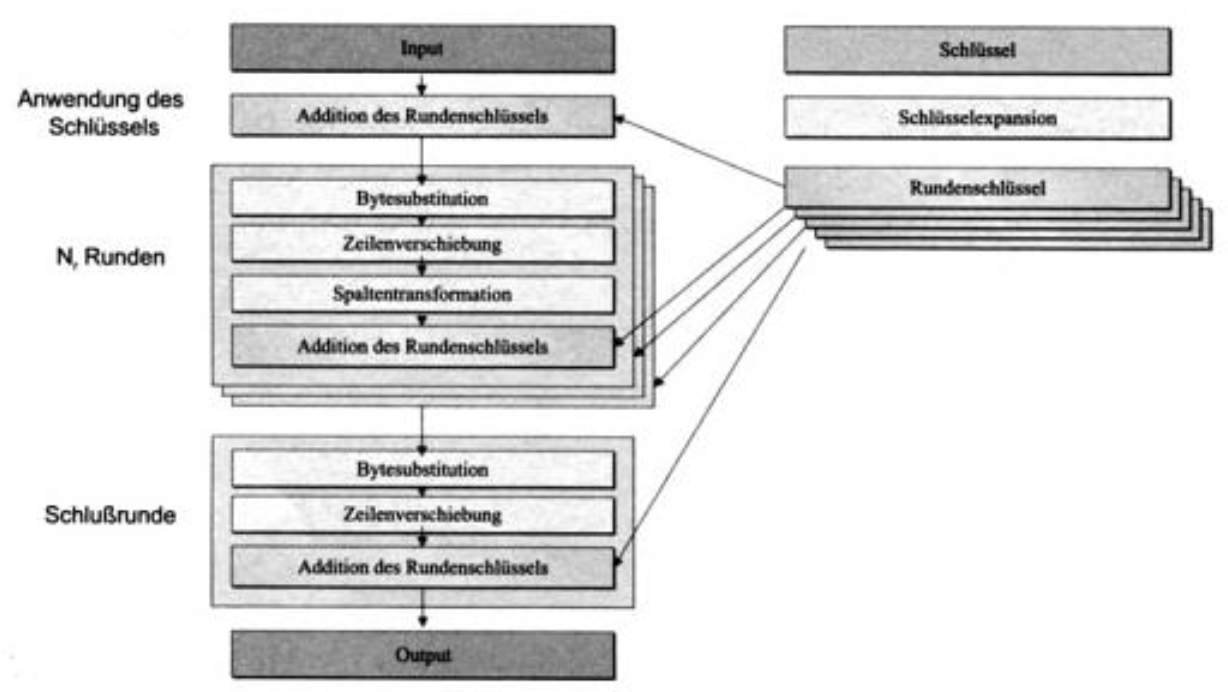
\includegraphics[width=0.40\textwidth]{Bilder/AES/AES_Schema}
	\caption{Schema des AES \citep{2}}
	\label{fig6}
\end{figure}
\noindent 
Beim AES wird der Text und die Ergebnisse als Bytes in eine 4x4-Matrix, in sogenannte States, gespeichert. Die Einträge erfolgen spaltenweise, wobei von links nach rechts angeordnet wird. Bei dieser Transformationsfunktion werden die 128 Bit in 16 Bytes geteilt. Diese Bytes werden als States in der Matrix bezeichnet. Die Suche erfolgt mittels der Indexe.
\cite{2}\cite{3}
\begin{figure}[H]
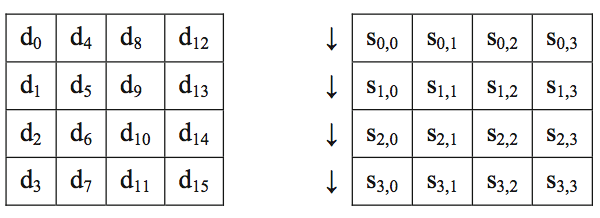
\includegraphics[width=0.40\textwidth]{Bilder/AES/AES_State}
	\caption{Datenstruktur: ein State \citep{3}}
	\label{fig7}
\end{figure}
\noindent
Wie auch DES eine Rundenfunktion besitzt, hat AES ebenfalls eine. Diese besteht aus SubBytes, ShiftRow, MixColumn und AddRoundKey. ??? 2.S.85
\cite{2}
% Kryptografie in Theorie und Praxis 7.7
% Kryptograhie und IT-Sicherheit 2.6

% Moderne Kryptographie 4.5

\subsubsection{IDEA (International Data Encryption Algorithm)}
\label{sec:international-data-encryption-algorithm}
% Kryptograhie und IT-Sicherheit 2.3

\subsection{Der RSA-Algorithmus}
\label{sec:rsa-algorithmus}
% Praktische Kryptographie unter Linux 2.4.3
% Kryptografie in Theorie und Praxis 10
% Kryptologie 5.3.4
% Kryptograhie und IT-Sicherheit 4.2
% Moderne Kryptographie 6.4
% Sicherheit und Kryptographie im Internet 1.5.4
% Verteilte Systeme S.430

\subsubsection{Schlüsselerzeugung}
\label{sec:key-generation}

\subsubsection{Verschlüsseln}
\label{sec:rsa-encrypt}

\subsubsection{Entschlüsseln}
\label{sec:rsa-decrypt}

\section{SSL/TLS-Protokoll}
\label{sec:ssl/tls-protocol}
% Praktische Kryptographie unter Linux 8.1
% Kryptograhie und IT-Sicherheit 6.3
% Sicherheit und Kryptographie im Internet 7.7/7.9
% Verteilte Systeme S.626

\subsection{SSL/TLS Grundlagen}
\label{sec:ssl-tls-basics}

\subsection{SSL/TLS im Protokollstapel}
\label{sec:ssl-tls-protocolstack}

\subsection{Client-Server-Kommunikation}
\label{sec:client-server-communication}



\subsection{Das SSL-Handshake}
\label{sec:ssl-handshake}

\subsection{TLS asymetrisch}
\label{sec:tls-asymetric}

\subsection{TLS symetrisch}
\label{sec:tls-symetric}

\subsection{TLS hybrid}
\label{sec:tls-hybrid}

\subsection{TLS Algorithmen}
\label{sec:tls-algorithmen}


\section{Schwierigkeiten bei Software}
\label{sec:sw-trouble}

\subsection{Buffer Ovrflow}
\label{sec:buffer-overflow}
% Improving Intrusion Detection Systems 4.3
% Network Intrusion Detection and Prevention 1.3.1

\subsection{OpenSSL}
\label{sec:openssl}
% Praktische Kryptographie unter Linux 8.2
% Sicherheit und Kryptographie im Internet 7.10

\newpage
\listoffigures
\addcontentsline{toc}{section}{Abbildungsverzeichnis}
\addcontentsline{toc}{section}{Literaturverzeichnis}
\mbox{}
\nocite{*}
\bibliographystyle{unsrt}
\bibliography{literatur}

\end{document}